\newpage
\begin{tcolorbox}
	


\chapter{2014 - Zkosi Zrcalo}
		\lettrine{I}{n} many ways the 2014 expedition adopted from the previous year's format. The duration of expedition was set at 5 weeks, between 11th of July and 14th August and in total 22 cavers made their pilgrimage to the hollow mountain, staying anywhere between 1 and 5 weeks. Camp \emph{X-Ray} in \emph{Friendship Gallery} as the chosen base for deep exploration. Most of the new passages visited this year were found south of \emph{Atlantis} and left as an expanding network of passages with many questions unanswered. The discovery of a large chamber and an active stream below made for a hydrological puzzle. 

		Hardy cavers were lured towards the deep end, where, after the discovery of the large series of rifts below Balamory, they headed down a winding stream passage until they met the water table at Aja! sump.  Due to the distance and hostility of the remaining 2013 pushing fronts, the feeling that some of the leads might be out of reach of the more novice cavers started had been circulating. In the end however, the discovery of 1.2km of cave, all of it at depths greater than 500m and sometimes as far as 3hrs from the camp, involved all the expedition's novices and dispelled any qualms about the accessibility of the pushing fronts.

 		The noteworthy visit to Colarado Sump a decade after its original discovery yielded, on top of its more obvious rerigging and rebolting by-products, an unexpected result: the previously 'terminal looking' sump revealed to be a mere duck. Jarvist Frost also put significant effort in laying the foundations for a deep, lightweight underground camp near \emph{Red Cow} with sights on \emph{Watership Down}, to this day the deepest point in the entire System.
		\\
		\\
		\\
		
\end{tcolorbox}
	\backgroundsetup{	scale=1,
					color=black,
					opacity=1,
					angle=0,
					contents={%
							  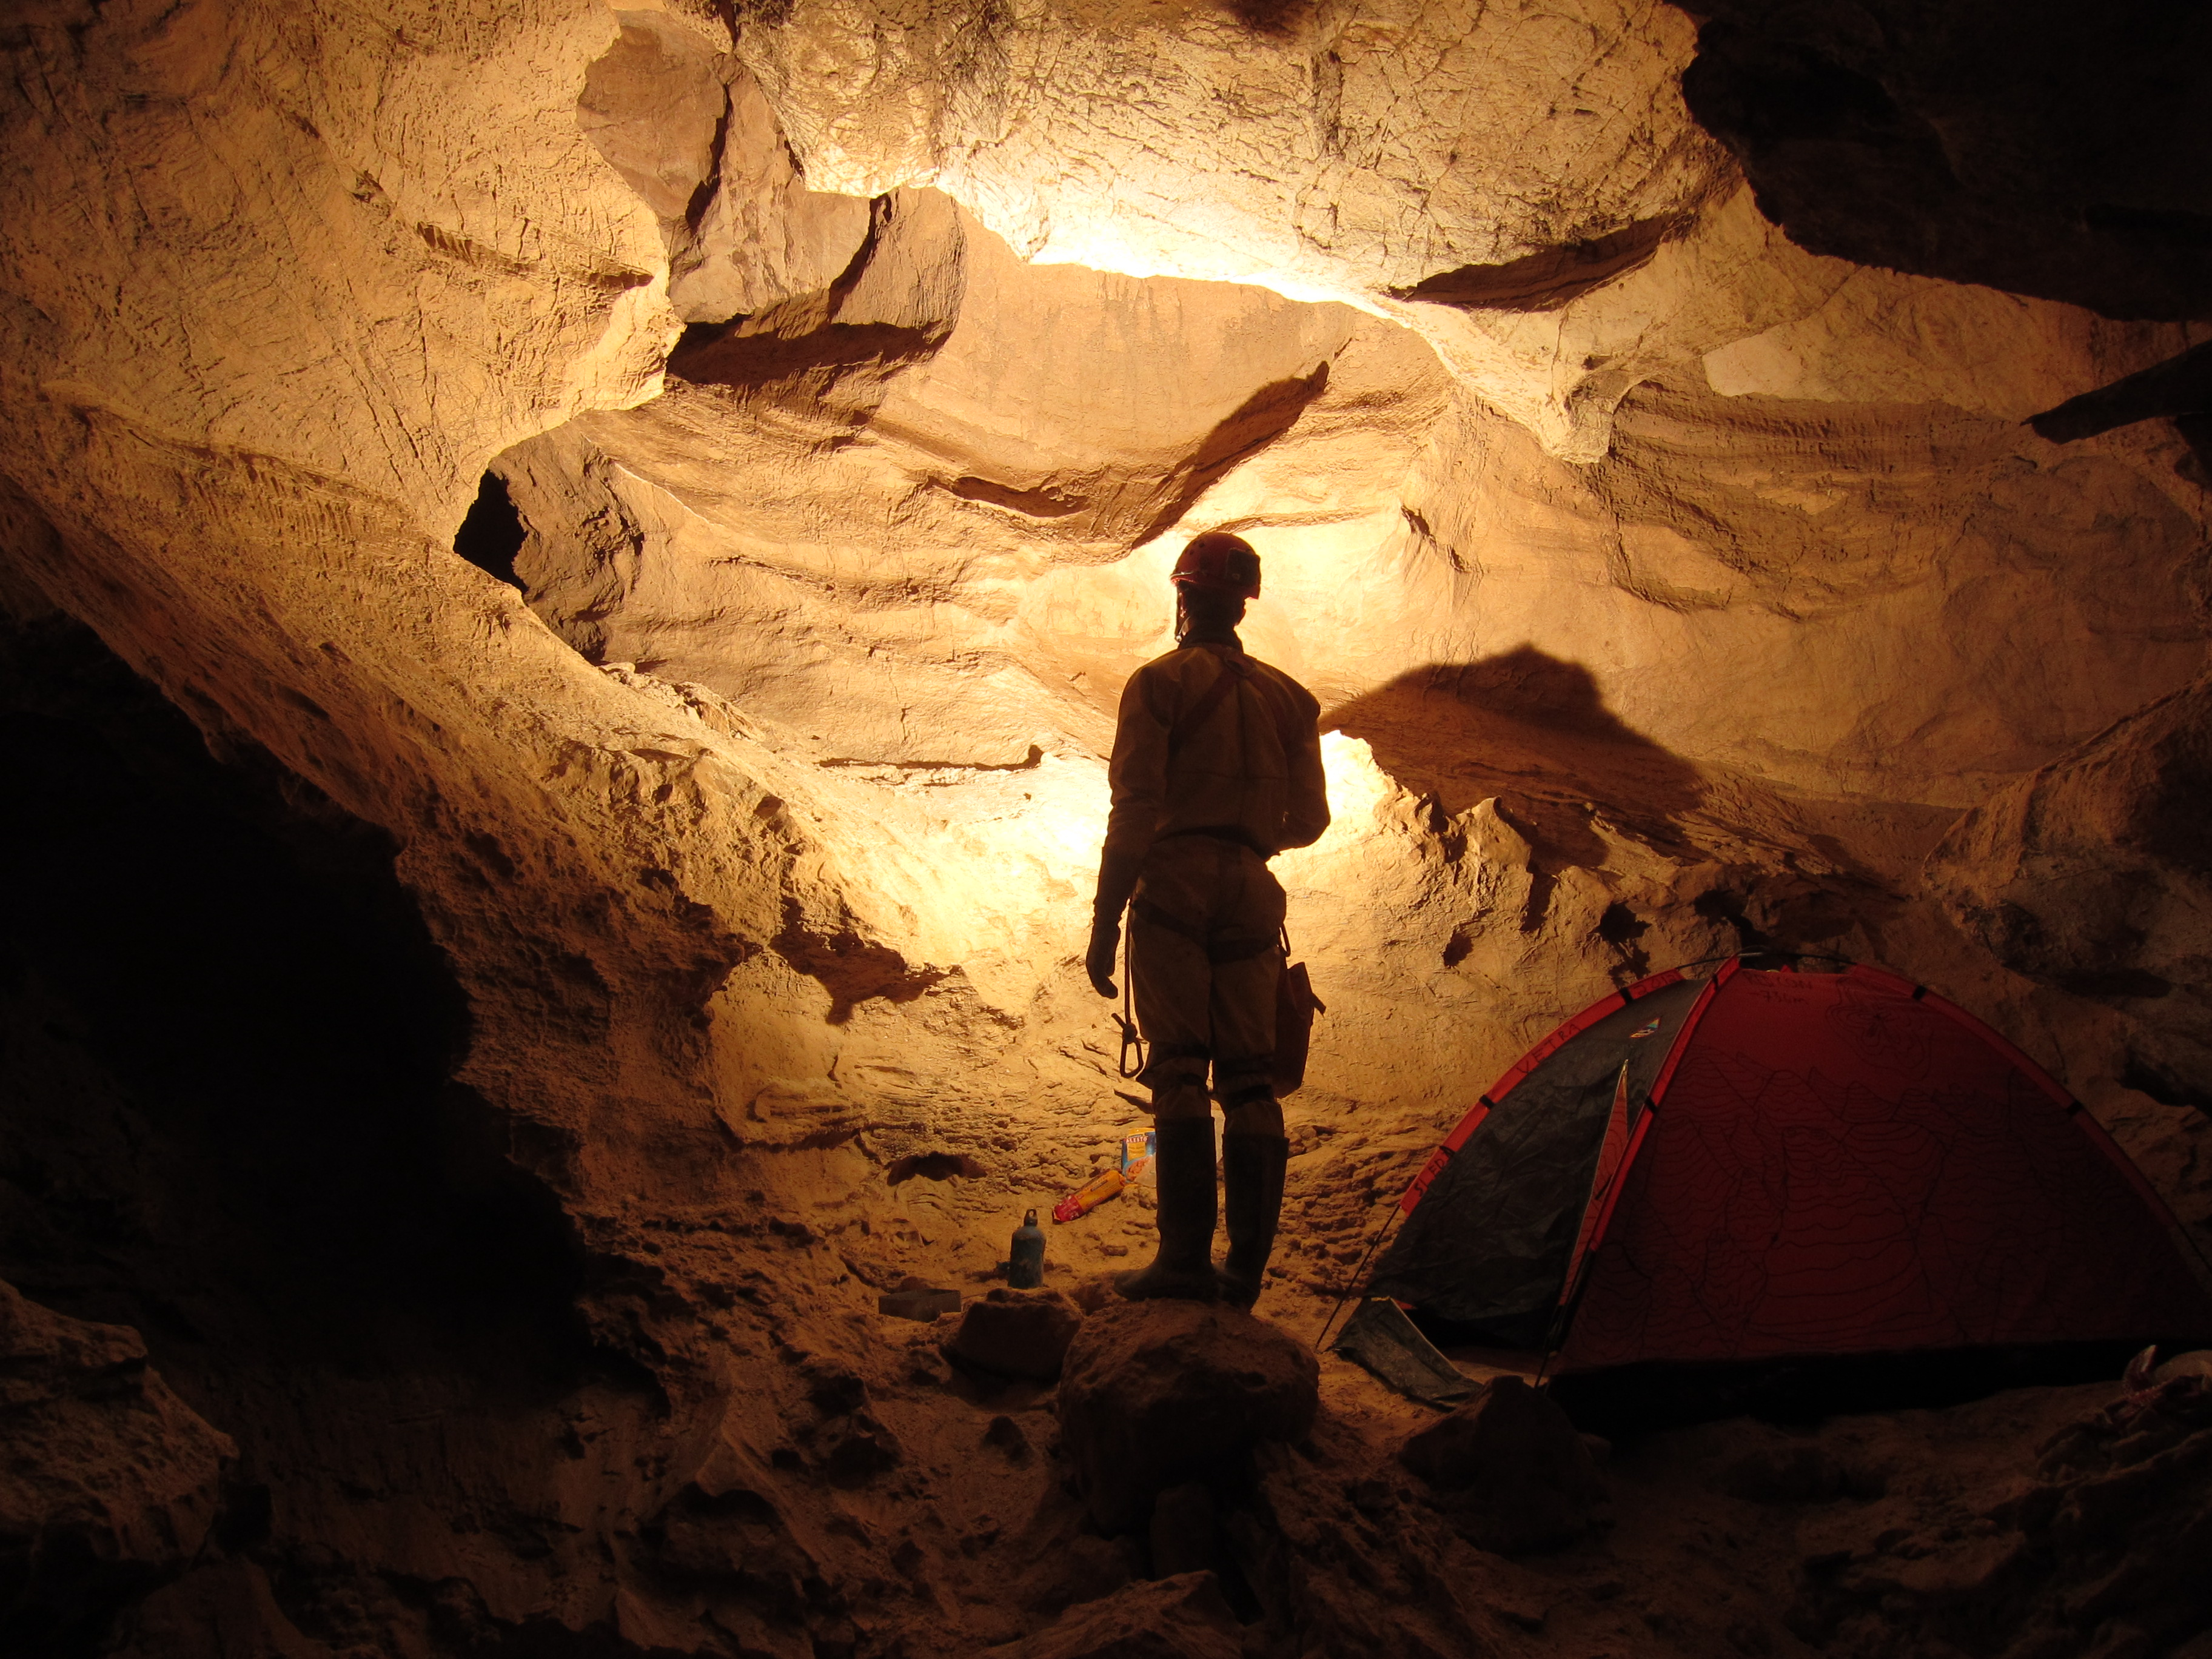
\includegraphics[height=\paperheight]{backgrounds/Rhys Red Cow.jpg}
 					 }
	}
\BgThispage